%%%%%%%%%%%%%%%%%%%%%%%%%%%%%%%%%%%%%%%%%%%%%%%%%%%%%%%%%%%%%%%%
%                                                              %
%                                                              %
% Macallyster S. Edmondson                                     %
%                                                              %
% ECE351-53                                                    %
%                                                              %
% Lab #5                                                       %
%                                                              %
% 02/22/2022                                                   %
%                                                              %
% Straightforward layout, broken into sections, uses many      %
% common libraries. Note, Hyperlinks are not highlighted.      %
%                                                              %
%%%%%%%%%%%%%%%%%%%%%%%%%%%%%%%%%%%%%%%%%%%%%%%%%%%%%%%%%%%%%%%%

%%%%%%%%%%%%%%%%%%%%%%%%%%%%%%%%%%%%%%%%%%%
%%% DOCUMENT PREAMBLE %%%
\documentclass[12pt]{report}
\usepackage[english]{babel}
%\usepackage{natbib}
\usepackage{url}
\usepackage[utf8x]{inputenc}
\usepackage{amsmath}
\usepackage{graphicx}
\graphicspath{{./images/}}
\usepackage{parskip}
\usepackage{fancyhdr}
\usepackage{vmargin}
\usepackage{listings}
\usepackage[hidelinks]{hyperref}
\usepackage{xcolor}
\usepackage[nodayofweek]{datetime}
\usepackage[section]{placeins}
\usepackage{pdfpages}
\definecolor{codegreen}{rgb}{0,0.6,0}
\definecolor{codegray}{rgb}{0.5,0.5,0.5}
\definecolor{codeblue}{rgb}{0,0,0.95}
\definecolor{backcolour}{rgb}{0.95,0.95,0.92}
\lstdefinestyle{mystyle}{
backgroundcolor=\color{backcolour},
commentstyle=\color{codegreen},
keywordstyle=\color{codeblue},
numberstyle=\tiny\color{codegray},
stringstyle=\color{codegreen},
basicstyle=\ttfamily\footnotesize,
breakatwhitespace=false,
breaklines=true,
captionpos=b,
keepspaces=true,
numbers=left,
numbersep=5pt,
showspaces=false,
showstringspaces=false,
showtabs=false,
tabsize=2
}
\lstset{style=mystyle}
\setmarginsrb{3 cm}{2.5 cm}{3 cm}{2.5 cm}{1 cm}{1 cm}{1 cm}{1.5 cm}
\title{Lab \#5 Report}
% Title
\author{Macallyster S. Edmondson}
% Author
\newdate{date}{22}{02}{2022}
\date{\longdate\displaydate{date}}
% Date
\makeatletter
\let\thetitle\@title
\let\theauthor\@author
\let\thedate\@date
\makeatother
\pagestyle{fancy}
\fancyhf{}
\rhead{\theauthor}
\lhead{\thetitle}
\lfoot{Page: \thepage}
\rfoot{\thedate}
\fancypagestyle{customplain}{ %Used for default pages with plain style to keep overall document consistency
  \fancyhf{}
  \renewcommand{\headrulewidth}{0pt} %Remove bar from top of page
  \lfoot{Page: \thepage}
}
\fancypagestyle{titlepage}{ %Used for default pages with plain style to keep overall document consistency
  \fancyhf{}
  \renewcommand{\headrulewidth}{0pt} %Remove bar from top of page
  \cfoot{\thedate}
}
\fancypagestyle{customblank}{ %Used for default pages with plain style to keep overall document consistency
  \fancyhf{}
  \renewcommand{\headrulewidth}{0pt} %Remove bar from top of page
}
%%%%%%%%%%%%%%%%%%%%%%%%%%%%%%%%%%%%%%%%%%%%
\begin{document}
%%%%%%%%%%%%%%%%%%%%%%%%%%%%%%%%%%%%%%%%%%%%%%%%%%%%%%%%%%%%%%%%%%%%%%%%%%
%%%%%%%%%%%%%%%
\begin{titlepage}\thispagestyle{titlepage}
\centering
%\vspace*{0.5 cm}

\includegraphics[scale = 0.12]{univ-logo.png}\\[1.0 cm]
%University of Idaho
\begin{center}    \textsc{\Large   ECE 351 - Section \#53 }\\[2.0 cm]
\end{center}% University Name

%Lab Report
\rule{\linewidth}{0.2 mm} \\[0.4 cm]
{ \huge \bfseries \thetitle}\\
\rule{\linewidth}{0.2 mm} \\[0.5 cm]
\textsc{\Large Step \& Impulse Response of a RLC Band Pass Filter }\\[1.5 cm] % Course 
\begin{minipage}{0.4\textwidth}
\begin{flushleft} \large
\emph{Submitted To:}\\
Kate Antonov\\ \small
University of Idaho\\
kantonov@uidaho.edu\\
\hfill
\end{flushleft}
\end{minipage}~
\begin{minipage}{0.4\textwidth}
\begin{flushright} \large
\emph{Submitted By :} \\
\theauthor \\ \small
University of Idaho\\
edmo7033@vandals.uidaho.edu\\
\href{http://github.com/mac-edmondson}{github.com/mac-edmondson}\\
\end{flushright}
\end{minipage}\\[2 cm]
\vfill
\end{titlepage}
%%%%%%%%%%%%%%%%%%%%%%%%%%%%%%%%%%%%%%%%%%%%%%%%%%%%%%%%%%%%%%%%%%%%%%%%%%
%%%%%%%%%%%%%%%
\tableofcontents\thispagestyle{customplain}
\pagebreak
%%%%%%%%%%%%%%%%%%%%%%%%%%%%%%%%%%%%%%%%%%%%%%%%%%%%%%%%%%%%%%%%%%%%%%%%%%
%%%%%%%%%%%%%%%
\renewcommand{\thesection}{\arabic{section}}
\section{Introduction}
The goal of this weeks lab was to use Laplace Transforms to find the time-domain response of an RLC bandpass filter using an impulse and step function as inputs.
This lab was a great introduction to plotting impulse and step responses based on an s-domain transfer function. The impulse response of the RLC circuit calculated
by the \texttt{scipy.signal.impulse()} function was double checked by plotting the hand-calculated time-domain impulse response. (More on this in \ref{Section: Part1}.)
Yet again, this lab was completed using \textit{Python} through the \textit{Spyder-IDE}. The packages used in the completion of this lab were \texttt{numpy} for 
definitions of mathematical functions, \texttt{matplotlib.pyplot} to plot outputs of functions, and \texttt{scipy.signal} to perform the impulse and step response of the
found s-domain transfer function for the RLC circuit from the preliminary.

All code for this lab, including this report, can be found on \href{http://github.com/mac-edmondson}{my Github}.
\section{Equations}\label{section: eq}
The equations used within this lab are shown in this section. The equations will be referenced by number throughout the rest of the report.
\begin{equation}\label{eq: 1}
  \begin{aligned}[c]
    R = 1\;k\Omega\; , L = 27\;mH\; , C = 100\;nF\\
  \end{aligned}
\end{equation}
\begin{equation}\label{eq: 2}
  \begin{aligned}[c]
    H(S) = \frac{L\cdot s}{R\cdot L\cdot C\cdot s^2 + L\cdot s + R} \; \textrm{ for values given in \eqref{eq: 1}}
  \end{aligned}
\end{equation}
\begin{equation}\label{eq: 3}
  \begin{aligned}
    h(t) = 10,000\cdot e^{-5,000t}\cdot (\cos{(18584.1t)} - 0.269\sin{(18584.1t)})u(t)
  \end{aligned}
\end{equation}
\begin{equation}\label{eq: 4}
  \begin{aligned}
    \textrm{FVT: } \lim_{t\to\infty} f(t) = \lim_{s\to 0} sF(s) \;\textrm{If all poles of } sF(s) \; \textrm{are in LHP.}
  \end{aligned}
\end{equation}

Note, Equations \eqref{eq: 1} - \eqref{eq: 3} are derived from the preliminary found in the \nameref{section: Attachments} section of this report. The preliminary
contains the RLC circuit, hand calculations, etc.

\section{Methodology}
\subsection{Lab: Part 1}\label{Section: Part1}
Part 1 of this lab was very simple. The code implemented for this part of the lab plots the impulse response based on the hand-calculated time-domain function found
for the preliminary circuit, Equation \eqref{eq: 3}, as well as the impulse response based on the hand-calculated s-domain function in which the time-domain function
was derived from, Equation \eqref{eq: 2}. Plotting the time-domain function was as simple as making a function of t and plotting the output as we have seen in many
prior labs. Plotting s-domain function involved making a system of coefficient matricies to then input into the \texttt{sig.impulse()} function, refer to \texttt{scipy.signal}
documentation for more information. As seen in the \nameref{section: Results} section, each of the two plots look identical, as expected.

Below can be seen the code implementation of the tasks carried out in Part 1 of this lab.

\begin{lstlisting}[language=Python, basicstyle=\footnotesize]
  #PART 1
  #1/2
  def h(t) :
  h = 10e3*np.exp(-5000*t)*(np.cos(18584.1*t) - (0.269 * np.sin(18584.1*t)))
  return h

  L = 27.0e-3   #H
  C = 100.0e-9  #F
  R = 1.0e3     #Ohms

  system = ([0, L, 0], [R*C*L, L, R])

  t = np.arange(0, 1.2e-3 + step_size, step_size)
  y1 = h(t)        

  tout, y2 = spsig.impulse(system, T=t);

  #Plot...
\end{lstlisting}

\subsection{Lab: Part 2}
In Part 2 of this lab, the goal was to use the \texttt{scipy.signal.step()} function to plot the step response of the s-domain transfer function found in the 
preliminary, Equation \eqref{eq: 2}. The implementation for this code was very simple and can be seen in the below listing.

\begin{lstlisting}[language=Python, basicstyle=\footnotesize]
  # PART 2
  # 1

  tout, y = spsig.step(system, T=t)

  plt.figure(figsize = (10, 11))
  plt.subplot(1, 1, 1)
  plt.plot(tout, y, "b-")
  plt.grid()
  plt.title('(h(t) * u(t)) v. t')
  plt.xlabel('t')
  plt.ylabel('Step Response of h(t)')
  plt.show()

  #Plot...
\end{lstlisting}

Additionally this part of the lab had us use the Final Value Theorem (FVT), seen in Equation \eqref{eq: 4}, to determine if the results from the plot generated from the above code make sense.
Using the FVT, the results of plot \ref{fig: p2t1} make perfect sense as the FVT tells us that the $\lim_{t\to\infty}(h(t)*u(t)) = 0$. Work seen in \nameref{section: Attachments} section.

\section{Results}\label{section: Results}
The results of this lab are very straightforward. The implementation of all functions worked as expected and the results are as expected.

The deliverables for Parts 1 \& 2 of this lab can be seen in Figures \ref{fig: p1t1} \& \ref{fig: p2t1}, below.
\\
\begin{figure}[h!]
  \centering
  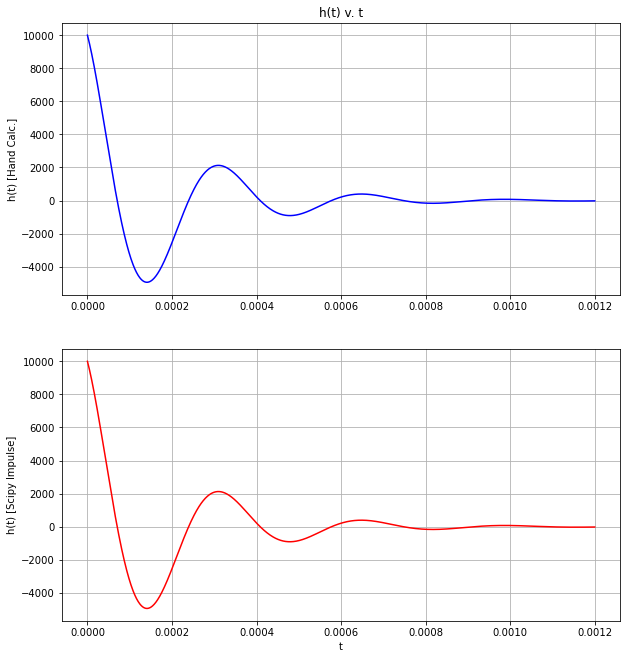
\includegraphics[scale=0.5]{p1t1.png}
  \caption{Part 1, Task 1 - Plots of RLC Impulse Response using Eqts. \eqref{eq: 3} \& \eqref{eq: 2}}
  \label{fig: p1t1}
\end{figure}
\begin{figure}[h!]
  \centering
  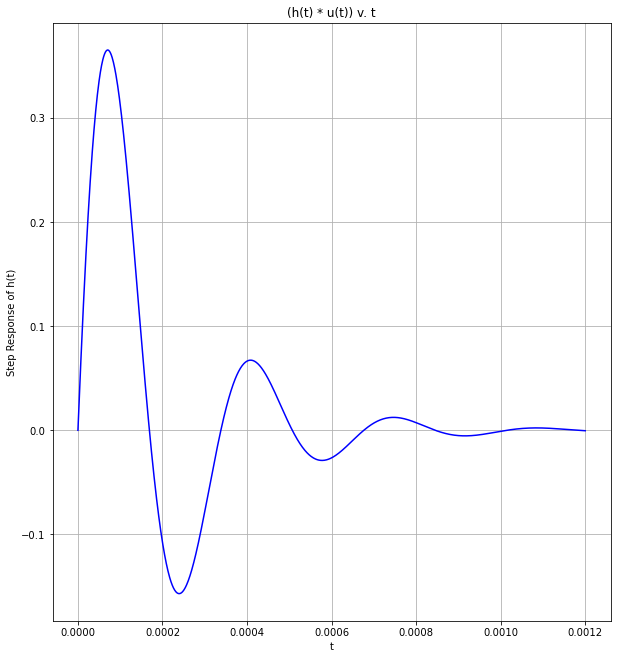
\includegraphics[scale=0.5]{p2t1.png}
  \caption{Part 2, Task 1 - Plot of RLC Step Response using Eq. \eqref{eq: 2}}
  \label{fig: p2t1}
\end{figure}
\section{Error Analysis}\label{section: ErAn}
No sources of error were seen or problems were encountered throughout the duration of this lab. 
\section{Questions}
\begin{enumerate}
  \item As known from the FVT used in Part 2 of this lab, the step response of the RLC circuit presented in this lab will approach 0 as $t\to\infty$. By simply
  looking at the circuit seen in the \nameref{section: Attachments} section of this report, this makes perfect sense. With an initial input, at an instant in time,
  there will be a small gain before the L \& C components reach a steady state and the gain of the componenents goes to 0. As seen in Figure \ref{fig: p2t1}, this all
  happens very quickly as the values of the components are very small, Eqts. \eqref{eq: 1} \& \eqref{eq: 2}. 
  \item This lab and its tasks were very concise in what is expected for deliverables. The preliminary work fit perfectly with not only what the lab was about,
  but also what we have been covering in class.
\end{enumerate}
\section{Conclusion}
In conclusion, I feel this lab was very successful. The implementation of the code in this lab was quite simple and I really enjoyed seeing how accurate the 
\texttt{scipy.signal} functions were as compared to hand calculated functions. All in all, I am very satisfied with what this lab has taught me and feel it was an excellent use of time.
\newpage
\thispagestyle{customblank}
\section{Attachments}\label{section: Attachments}
\centering\begin{enumerate}
  \item Pre-Lab
  \item FVT Calculations
\end{enumerate}
\vspace*{\fill}

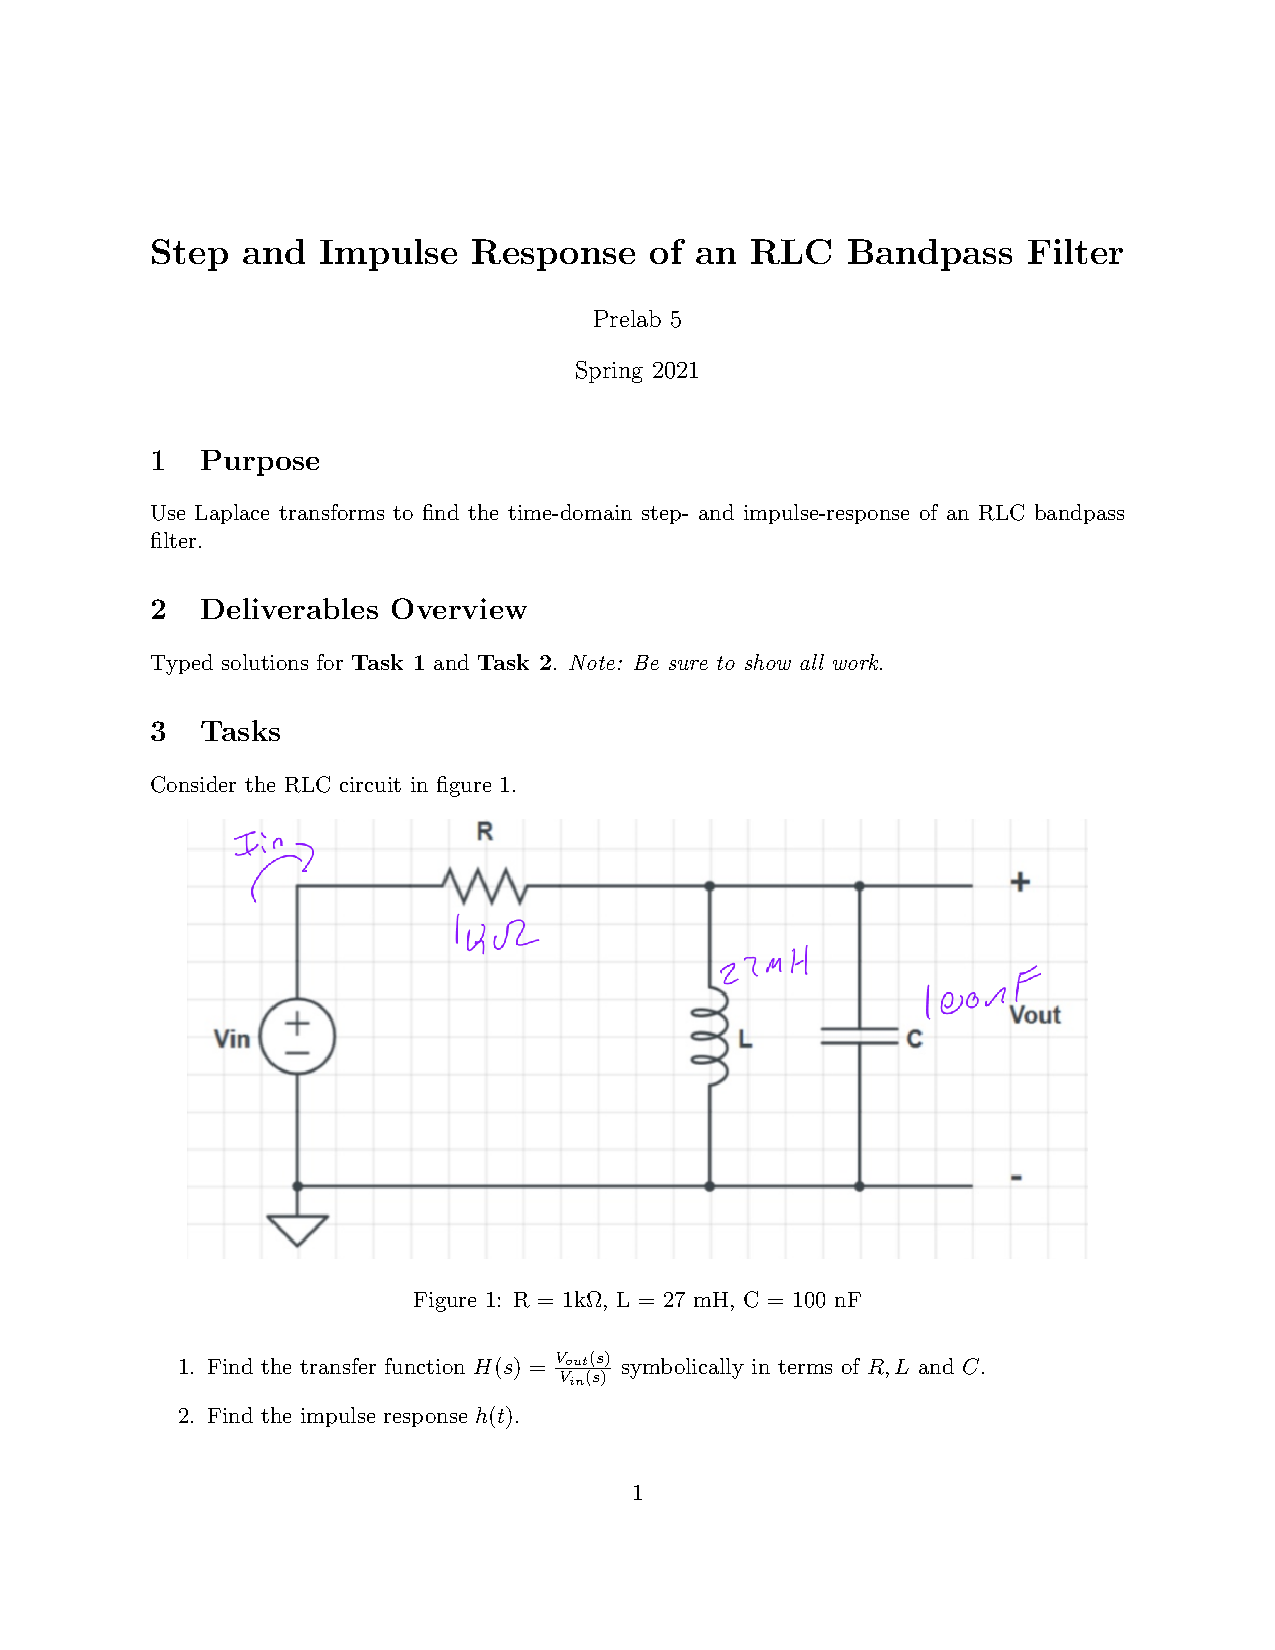
\includepdf[pages=-, offset=1in -1in]{./attachments/lab5_pre.pdf}
\includepdf[pages=3, offset=1in -1in]{./attachments/lab5.pdf}

% \begin{thebibliography}{111}
% \thispagestyle{customplain}

% \end{thebibliography}
\end{document}
%This template was created by Roza Aceska.